\documentclass[12pt,a4paper]{article}

% ── Paquetes ──
\usepackage[utf8]{inputenc}
\usepackage[spanish]{babel}
\usepackage[left=2.5cm,right=2.5cm,top=2.5cm,bottom=3cm]{geometry}
\usepackage{float}
\usepackage{graphicx}
\usepackage{enumitem}
\usepackage{booktabs}
\usepackage{amsmath,amssymb}
\usepackage[hidelinks]{hyperref}
\usepackage{parskip}
\usepackage{caption}
\usepackage{subcaption}
\usepackage{listings}
\usepackage{xcolor}
\usepackage{fancyhdr}
\usepackage{titlesec}

\setlength{\parindent}{1.27cm}

% ── Estilo de código ──
\definecolor{codebg}{HTML}{F5F5F5}
\definecolor{codeframe}{HTML}{CCCCCC}
\definecolor{codecomment}{HTML}{6A9955}
\definecolor{codestring}{HTML}{CE9178}
\definecolor{codekeyword}{HTML}{569CD6}

\lstset{
  language=Python,
  basicstyle=\ttfamily\small,
  backgroundcolor=\color{codebg},
  frame=single,
  rulecolor=\color{codeframe},
  keywordstyle=\color{codekeyword}\bfseries,
  commentstyle=\color{codecomment}\itshape,
  stringstyle=\color{codestring},
  showstringspaces=false,
  breaklines=true,
  numbers=left,
  numberstyle=\tiny\color{gray},
  numbersep=8pt,
  tabsize=4,
  captionpos=b,
  aboveskip=1em,
  belowskip=1em,
}

% ── Encabezados y pies ──
\pagestyle{fancy}
\fancyhf{}
\fancyhead[L]{\small\textit{Coeficiente de Restitución — Visión Computacional}}
\fancyhead[R]{\small\textit{UTB}}
\fancyfoot[C]{\thepage}
\renewcommand{\headrulewidth}{0.4pt}

% ── Formato de secciones ──
\titleformat{\section}{\Large\bfseries}{\thesection.}{0.5em}{}
\titleformat{\subsection}{\large\bfseries}{\thesubsection.}{0.5em}{}
\titleformat{\subsubsection}{\normalsize\bfseries}{\thesubsubsection.}{0.5em}{}

\begin{document}

% ════════════════════════════════════════════════════════════════
% PORTADA
% ════════════════════════════════════════════════════════════════
\begin{titlepage}
	\centering
	
\includegraphics[width=0.50\textwidth]{../../resources/logos/Nuevo-logo-UTB-1.png}\par\vspace{0.5cm}
	{\scshape\LARGE\textbf{Universidad Tecnológica de Bolívar} \par}
	\vspace{1.5cm}
	\rule{\linewidth}{0.2mm}\\[0.4cm]
	{\huge\bfseries Estimación del coeficiente de restitución \par}
	\rule{\linewidth}{0.2mm}\\[1.0cm]
	\vspace{0.5cm}

	{\large\textbf{Actividad 1 — Segundo corte} \par}
	\vspace{0.3cm}
	{\large Sensado y Modelado de Sistemas Físicos \par}
	\vspace{1.5cm}

	\centering{\emph{\textbf{Estudiantes:}}\\
		German De Armas Castaño \\
		Angel Vega Rodriguez \\
		Michael Taboada Naranjo\\}

	\vspace{1cm}
	\centering{\emph{\textbf{Profesor:}}\\
		David Sierra Porta\\}

	\vfill
	{\large \today\par}
\end{titlepage}

\tableofcontents
\newpage

% ════════════════════════════════════════════════════════════════
% 1. INTRODUCCIÓN
% ════════════════════════════════════════════════════════════════
\section{Introducción}

El presente reporte documenta el diseño, implementación y validación de un sistema automatizado para la estimación experimental del \textbf{coeficiente de restitución} ($e$) de un cuerpo que colisiona repetidamente contra una superficie rígida. El proyecto se desarrolló en dos fases claramente diferenciadas:

\begin{enumerate}[label=\textbf{\arabic*.}]
    \item \textbf{Fase de exploración y prototipado} — implementada íntegramente en un \textit{notebook} de Python (\texttt{restitution\_calculator.ipynb}), donde se diseñaron, probaron y validaron todos los algoritmos de visión computacional y procesamiento de señales.
    \item \textbf{Fase de productización} — los hallazgos del notebook se encapsularon en una aplicación web interactiva (React + FastAPI) integrada al ecosistema \textbf{Bento Launcher}, permitiendo que cualquier usuario reproduzca el análisis sin necesidad de escribir código.
\end{enumerate}

Este documento sigue la narrativa natural del flujo de trabajo: primero se exponen los fundamentos teóricos, luego se detalla paso a paso cómo se implementó cada etapa en el notebook, y finalmente se muestra cómo la aplicación web materializa dichos hallazgos en una interfaz accesible.

\subsection{Planteamiento del problema}

El coeficiente de restitución cuantifica la fracción de energía cinética que se conserva tras un impacto. Medirlo manualmente — observando a simple vista las alturas sucesivas de un objeto que rebota — introduce errores significativos debido a:

\begin{itemize}
    \item La \textbf{latencia de reacción humana}: el instante de altura máxima dura fracciones de segundo.
    \item El \textbf{sesgo de perspectiva}: la posición del observador distorsiona la lectura de alturas.
    \item La \textbf{falta de repetibilidad}: cada observador obtiene valores distintos.
\end{itemize}

Un sistema de visión computacional elimina estas fuentes de error al evaluar \textit{cada fotograma} del video, extrayendo la posición vertical del objeto con resolución sub-píxel y consistencia absoluta entre ejecuciones.

\subsection{Objetivos}

\begin{enumerate}[label=\textbf{\arabic*.}]
    \item Implementar un algoritmo de segmentación por color en el espacio HSV para aislar el objeto en cada fotograma del video.
    \item Extraer la serie temporal de la coordenada vertical ($Y$) del centroide del objeto a lo largo de todo el video.
    \item Aplicar detección de picos (\texttt{scipy.signal.find\_peaks}) con filtrado por prominencia para identificar las alturas máximas de cada rebote.
    \item Calcular el coeficiente de restitución promedio $\bar{e}$ y su desviación estándar $\sigma_e$ a partir de las alturas consecutivas.
    \item Encapsular el pipeline completo en una aplicación web desplegable desde el Bento Launcher.
\end{enumerate}

% ════════════════════════════════════════════════════════════════
% 2. FUNDAMENTOS TEÓRICOS
% ════════════════════════════════════════════════════════════════
\section{Fundamentos Teóricos}

\subsection{El coeficiente de restitución ($e$)}

El coeficiente de restitución es un escalar adimensional que relaciona las velocidades relativas antes y después de una colisión. En su forma general (Newton):

\begin{equation}
    e = \frac{v_{\text{sep}}}{v_{\text{aprox}}}
\end{equation}

donde $v_{\text{sep}}$ es la velocidad relativa de separación y $v_{\text{aprox}}$ la de aproximación. Para un objeto que rebota verticalmente contra el suelo, la conservación de energía mecánica (con disipación únicamente en el impacto) permite expresar $e$ en función de las alturas:

\begin{equation}
    \label{eq:restitution}
    e = \sqrt{\frac{h_{n+1}}{h_n}}
\end{equation}

donde $h_n$ es la altura máxima alcanzada en el rebote $n$-ésimo y $h_{n+1}$ la del rebote siguiente. Esta relación se deriva directamente de la equivalencia entre energía potencial gravitatoria y energía cinética en el punto de impacto:

\begin{align}
    v_n &= \sqrt{2 g h_n} \\
    v_{n+1} &= \sqrt{2 g h_{n+1}} \\
    e &= \frac{v_{n+1}}{v_n} = \sqrt{\frac{h_{n+1}}{h_n}}
\end{align}

El coeficiente $e$ toma valores en el intervalo $[0, 1]$:
\begin{itemize}
    \item $e = 0$: colisión perfectamente inelástica (toda la energía cinética se disipa).
    \item $e = 1$: colisión perfectamente elástica (no hay pérdida de energía).
\end{itemize}

Para un conjunto de $N$ rebotes detectados, se calcula el promedio:

\begin{equation}
    \bar{e} = \frac{1}{N-1} \sum_{i=1}^{N-1} \sqrt{\frac{h_{i+1}}{h_i}}
\end{equation}

\subsection{Espacio de color HSV y segmentación}

El espacio de color HSV (Hue, Saturation, Value) descompone el color en tres componentes perceptualmente intuitivos:

\begin{itemize}
    \item \textbf{Hue (H)}: el tono cromático, representado como un ángulo en $[0°, 360°]$ (en OpenCV se escala a $[0, 180]$).
    \item \textbf{Saturation (S)}: la pureza del color, en $[0, 255]$.
    \item \textbf{Value (V)}: la luminosidad, en $[0, 255]$.
\end{itemize}

A diferencia del espacio BGR/RGB, HSV permite aislar objetos por su tonalidad independientemente de las condiciones de iluminación, lo que lo hace ideal para la segmentación por color en escenas con iluminación variable.

La segmentación se realiza mediante un umbralizado por rango:

\begin{equation}
    \text{mask}(x, y) =
    \begin{cases}
        255 & \text{si } H_{\min} \leq H(x,y) \leq H_{\max} \;\land\; S_{\min} \leq S(x,y) \leq S_{\max} \;\land\; V_{\min} \leq V(x,y) \leq V_{\max} \\
        0   & \text{en caso contrario}
    \end{cases}
\end{equation}

\subsection{Operaciones morfológicas}

Tras la segmentación, la máscara binaria suele contener ruido (píxeles aislados falsos positivos) y huecos internos. Se aplican dos operaciones morfológicas secuenciales:

\begin{enumerate}
    \item \textbf{Apertura} (\texttt{MORPH\_OPEN}): erosión seguida de dilatación. Elimina pequeños objetos espurios sin alterar significativamente el contorno del objeto principal.
    \item \textbf{Cierre} (\texttt{MORPH\_CLOSE}): dilatación seguida de erosión. Rellena huecos internos en la máscara del objeto.
\end{enumerate}

Ambas operaciones utilizan un elemento estructurante elíptico de $5 \times 5$ píxeles.

\subsection{Cálculo del centroide mediante momentos espaciales}

Una vez obtenida la máscara limpia, se calculan los \textbf{momentos espaciales} de la región detectada. El centroide $(c_x, c_y)$ se obtiene como:

\begin{equation}
    c_x = \frac{M_{10}}{M_{00}}, \qquad c_y = \frac{M_{01}}{M_{00}}
\end{equation}

donde $M_{pq} = \sum_x \sum_y x^p \cdot y^q \cdot I(x,y)$ son los momentos de orden $(p, q)$ de la imagen binaria $I$.

\subsection{Detección de picos con \texttt{scipy.signal.find\_peaks}}

La serie temporal de alturas $h(t)$ se analiza con el algoritmo \texttt{find\_peaks} de SciPy, que identifica máximos locales sujetos a restricciones configurables:

\begin{itemize}
    \item \textbf{Prominencia} (\texttt{prominence}): altura mínima que un pico debe sobresalir respecto a sus valles adyacentes. Filtra oscilaciones menores causadas por ruido en la detección.
    \item \textbf{Distancia} (\texttt{distance}): separación mínima (en muestras) entre picos consecutivos. Evita la detección de picos duplicados en un mismo rebote.
\end{itemize}

% ════════════════════════════════════════════════════════════════
% 3. IMPLEMENTACIÓN EN EL NOTEBOOK
% ════════════════════════════════════════════════════════════════
\section{Implementación en el Notebook}

El notebook \texttt{restitution\_calculator.ipynb} estructura el análisis en cinco módulos funcionales que se ejecutan secuencialmente. A continuación se detalla cada uno.

\subsection{Módulo 1: Detección del objeto (\texttt{detect\_ball})}

La función \texttt{detect\_ball} recibe un fotograma y los umbrales HSV, y retorna el centroide del objeto detectado. El pipeline interno es:

\begin{enumerate}
    \item Conversión del fotograma de BGR a HSV mediante \texttt{cv2.cvtColor}.
    \item Generación de la máscara binaria con \texttt{cv2.inRange}.
    \item Limpieza morfológica: apertura y cierre con kernel elíptico $5 \times 5$.
    \item Búsqueda de contornos con \texttt{cv2.findContours}.
    \item Selección del contorno de mayor área (descartando áreas menores a \texttt{min\_area}$= 50$ px).
    \item Cálculo del centroide $(c_x, c_y)$ mediante momentos espaciales.
\end{enumerate}

\begin{lstlisting}[caption={Función de detección del objeto.}]
def detect_ball(frame, lower_hsv, upper_hsv, min_area=50):
    hsv = cv2.cvtColor(frame, cv2.COLOR_BGR2HSV)
    mask = cv2.inRange(hsv, lower_hsv, upper_hsv)

    kernel = cv2.getStructuringElement(cv2.MORPH_ELLIPSE, (5, 5))
    mask = cv2.morphologyEx(mask, cv2.MORPH_OPEN, kernel)
    mask = cv2.morphologyEx(mask, cv2.MORPH_CLOSE, kernel)

    contours, _ = cv2.findContours(
        mask, cv2.RETR_EXTERNAL, cv2.CHAIN_APPROX_SIMPLE)
    if not contours:
        return None, mask

    largest = max(contours, key=cv2.contourArea)
    if cv2.contourArea(largest) < min_area:
        return None, mask

    M = cv2.moments(largest)
    if M["m00"] == 0:
        return None, mask

    cx = int(M["m10"] / M["m00"])
    cy = int(M["m01"] / M["m00"])
    return (cx, cy), mask
\end{lstlisting}

\subsection{Módulo 2: Calibración interactiva HSV}

Antes de procesar el video completo, es necesario determinar los umbrales HSV que aíslan correctamente el objeto. El notebook implementa una interfaz interactiva con \texttt{cv2.createTrackbar} que permite:

\begin{itemize}
    \item Navegar por los fotogramas del video con un slider temporal.
    \item Ajustar en tiempo real los seis parámetros ($H_{\min}$, $H_{\max}$, $S_{\min}$, $S_{\max}$, $V_{\min}$, $V_{\max}$).
    \item Visualizar simultáneamente el fotograma original y la máscara binaria resultante.
    \item Confirmar la selección con la tecla \texttt{ENTER}.
\end{itemize}

Este paso es crítico: una calibración deficiente produce falsos positivos (ruido) o falsos negativos (pérdida del objeto), ambos degradando la calidad de la serie temporal.

\subsection{Módulo 3: Tracking frame-a-frame}

La función \texttt{process\_video\_tracking} recorre el video completo aplicando \texttt{detect\_ball} en cada fotograma. Para cada detección exitosa, registra:

\begin{itemize}
    \item El instante temporal $t = \text{frame\_idx} / \text{fps}$.
    \item La coordenada vertical $Y$ del centroide.
\end{itemize}

El resultado es un par de arrays NumPy: \texttt{time\_series} y \texttt{y\_series}, que conforman la señal cruda de posición vertical vs. tiempo.

\begin{lstlisting}[caption={Extracción de la serie temporal $Y(t)$.}]
def process_video_tracking(video_path, lower_hsv, upper_hsv):
    cap = cv2.VideoCapture(video_path)
    fps = cap.get(cv2.CAP_PROP_FPS)
    time_series, y_series = [], []

    frame_idx = 0
    while True:
        ret, frame = cap.read()
        if not ret:
            break
        center, _ = detect_ball(frame, lower_hsv, upper_hsv)
        if center:
            t = frame_idx / fps
            time_series.append(t)
            y_series.append(center[1])
        frame_idx += 1

    cap.release()
    return np.array(time_series), np.array(y_series)
\end{lstlisting}

\subsection{Módulo 4: Cálculo del coeficiente de restitución}

La función \texttt{compute\_restitution} transforma la señal cruda en alturas relativas y extrae los picos correspondientes a cada rebote. El procedimiento es:

\subsubsection{Paso 1: Determinación del nivel del suelo}

En el sistema de coordenadas de OpenCV, el eje $Y$ crece hacia abajo. Por lo tanto, el ``suelo'' corresponde al valor máximo de $Y$ en la serie. Se utiliza el percentil 98 para robustez frente a valores atípicos:

\begin{equation}
    Y_{\text{piso}} = P_{98}(Y)
\end{equation}

\subsubsection{Paso 2: Conversión a alturas relativas}

La altura sobre el suelo en cada instante se calcula como:

\begin{equation}
    h(t) = Y_{\text{piso}} - Y(t)
\end{equation}

\subsubsection{Paso 3: Detección de picos}

Se aplica \texttt{find\_peaks} sobre $h(t)$ con los parámetros:
\begin{itemize}
    \item \texttt{prominence} $= 20$ px: descarta oscilaciones menores.
    \item \texttt{distance} $= 5$ frames: evita picos duplicados.
\end{itemize}

\subsubsection{Paso 4: Cálculo iterativo de $e$}

Para cada par de picos consecutivos $(h_i, h_{i+1})$, se aplica la ecuación~\eqref{eq:restitution} con un filtro de seguridad: solo se consideran pares donde $h_{i+1} < h_i$ (el rebote siguiente debe ser menor que el anterior, descartando anomalías por ruido o viento).

\begin{lstlisting}[caption={Cálculo del coeficiente de restitución.}]
def compute_restitution(time_series, y_pixels):
    y_floor = np.percentile(y_pixels, 98)
    heights = y_floor - y_pixels

    peaks_indices, _ = find_peaks(
        heights, prominence=20, distance=5)
    peak_times = time_series[peaks_indices]
    peak_heights = heights[peaks_indices]

    coefficients = []
    for i in range(len(peak_heights) - 1):
        h_n = peak_heights[i]
        h_next = peak_heights[i + 1]
        if h_next < h_n and h_n > 0:
            e = np.sqrt(h_next / h_n)
            coefficients.append(e)

    avg_e = np.mean(coefficients) if coefficients else 0
    std_e = np.std(coefficients) if coefficients else 0
    return avg_e, std_e, peak_times, peak_heights
\end{lstlisting}

\subsection{Módulo 5: Visualización de resultados}

El notebook genera una gráfica consolidada (Figura~\ref{fig:restitution-plot}) que superpone:

\begin{itemize}
    \item La señal completa de altura relativa $h(t)$ (línea azul).
    \item Los picos detectados marcados con cruces rojas y anotados con su altura en píxeles.
    \item El título incluye el valor calculado de $\bar{e} \pm \sigma_e$.
\end{itemize}

\begin{figure}[H]
    \centering
    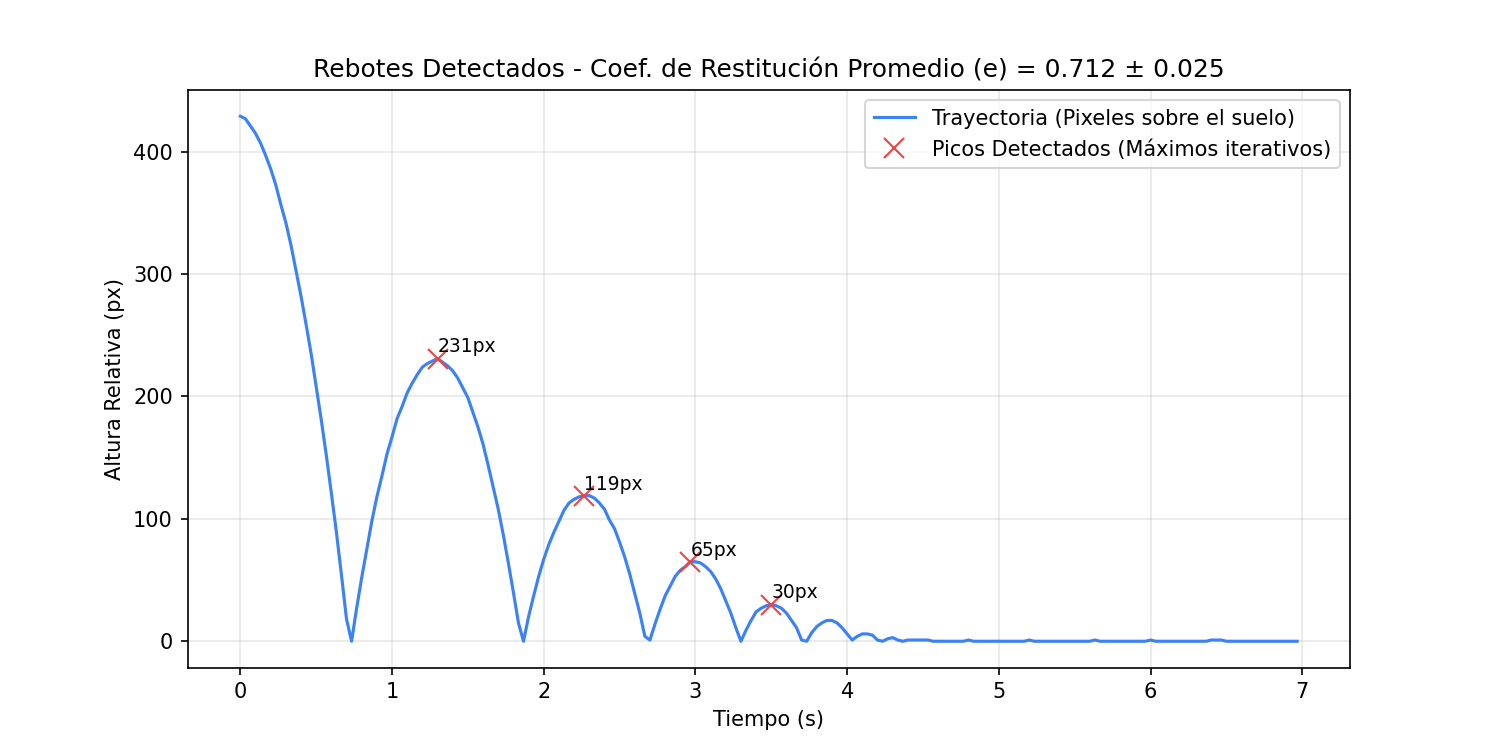
\includegraphics[width=0.85\linewidth]{imgs/restitution_plot.png}
    \caption{Gráfica generada por el notebook: trayectoria de alturas con picos detectados y coeficiente de restitución calculado.}
    \label{fig:restitution-plot}
\end{figure}

% ════════════════════════════════════════════════════════════════
% 4. APLICACIÓN WEB — BENTO LAUNCHER
% ════════════════════════════════════════════════════════════════
\section{Aplicación Web en el Bento Launcher}

Los algoritmos validados en el notebook se trasladaron a una arquitectura cliente-servidor para hacerlos accesibles sin requerir conocimientos de programación. La aplicación se integra al ecosistema \textbf{Bento Launcher}, un hub central que orquesta el arranque de todos los módulos del repositorio.

\subsection{Arquitectura}

\begin{itemize}
    \item \textbf{Backend} (FastAPI, puerto 8002): expone un endpoint de streaming que ejecuta el motor de procesamiento (\texttt{engine.py}) y transmite el progreso frame a frame al cliente mediante Server-Sent Events.
    \item \textbf{Frontend} (React + Vite, puerto 5175): interfaz interactiva con paneles de carga de video, calibración HSV visual, visualización de trayectoria y presentación de resultados.
\end{itemize}

\subsection{Lanzamiento desde el Bento Launcher}

El flujo inicia desde el menú central del Bento Launcher. Al seleccionar la tarjeta ``Coeficiente de Restitución'', el sistema orquesta automáticamente el arranque del backend y el frontend, mostrando el progreso en una terminal integrada.

\begin{figure}[H]
    \centering
    \begin{subfigure}[b]{0.48\textwidth}
        \centering
        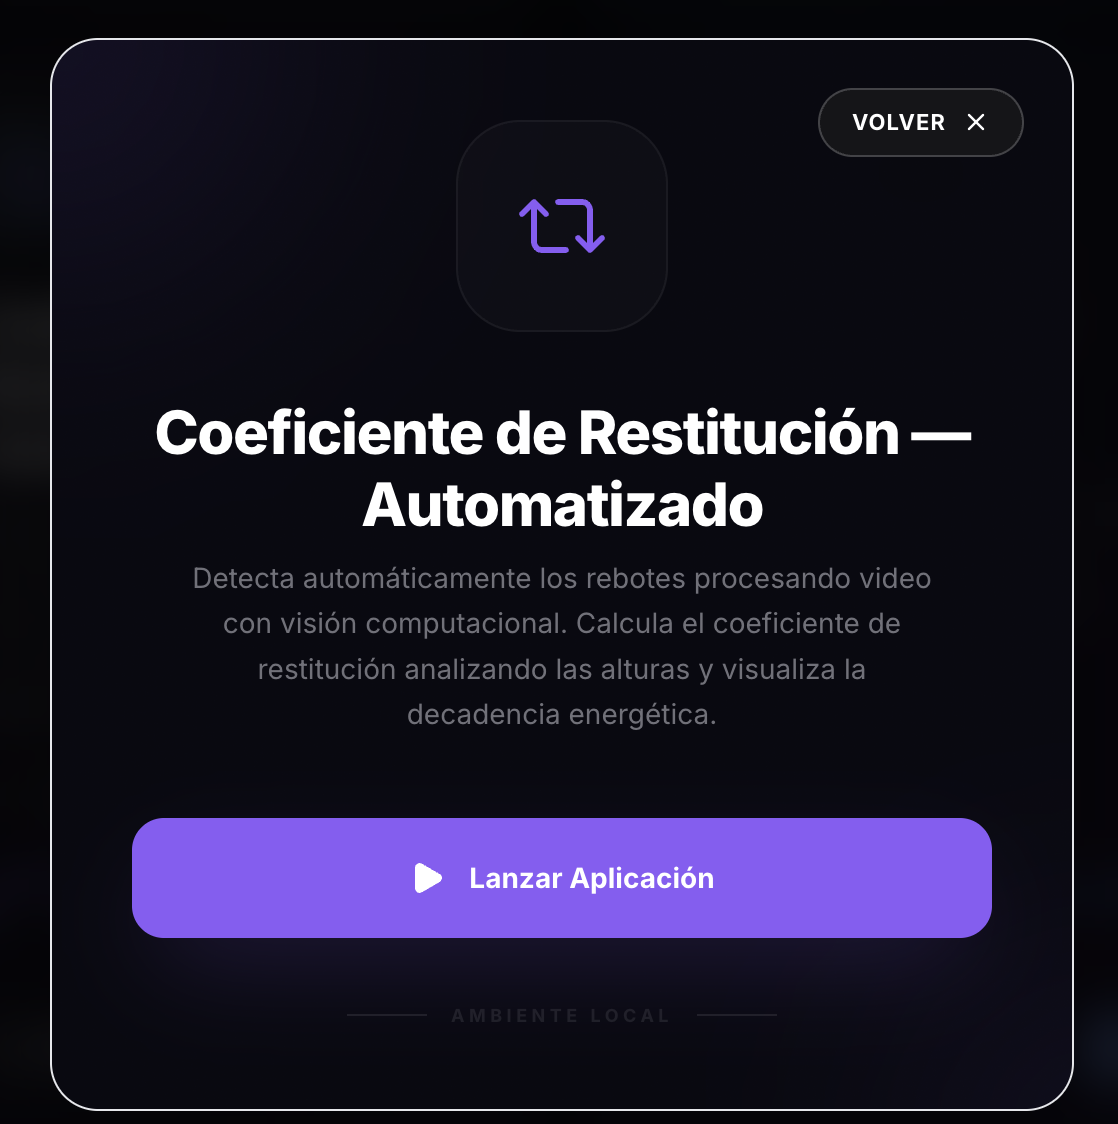
\includegraphics[width=0.9\linewidth]{imgs/lanzar-app.png}
        \caption{Tarjeta de la app en el Bento Launcher.}
        \label{fig:bento-card}
    \end{subfigure}
    \hfill
    \begin{subfigure}[b]{0.48\textwidth}
        \centering
        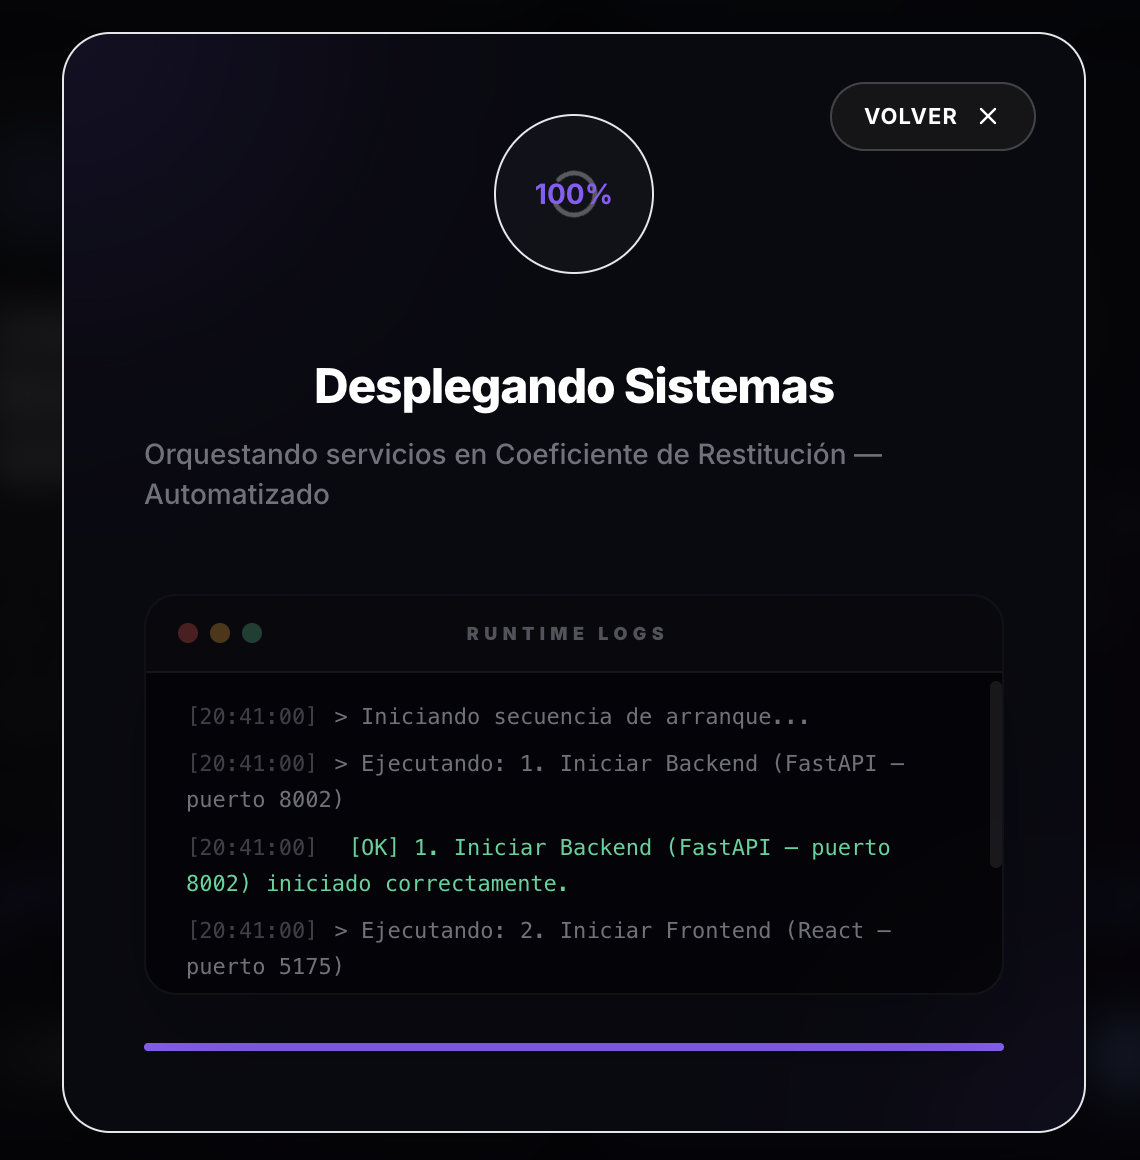
\includegraphics[width=0.9\linewidth]{imgs/procesos-arranque.png}
        \caption{Terminal de arranque automatizado.}
        \label{fig:bento-launch}
    \end{subfigure}
    \caption{Lanzamiento de la aplicación desde el ecosistema Bento.}
\end{figure}

\subsection{Carga del video}

Una vez activa la aplicación, el usuario accede a un panel donde puede cargar el archivo de video a procesar. La interfaz valida el formato y muestra una vista previa.

\begin{figure}[H]
    \centering
    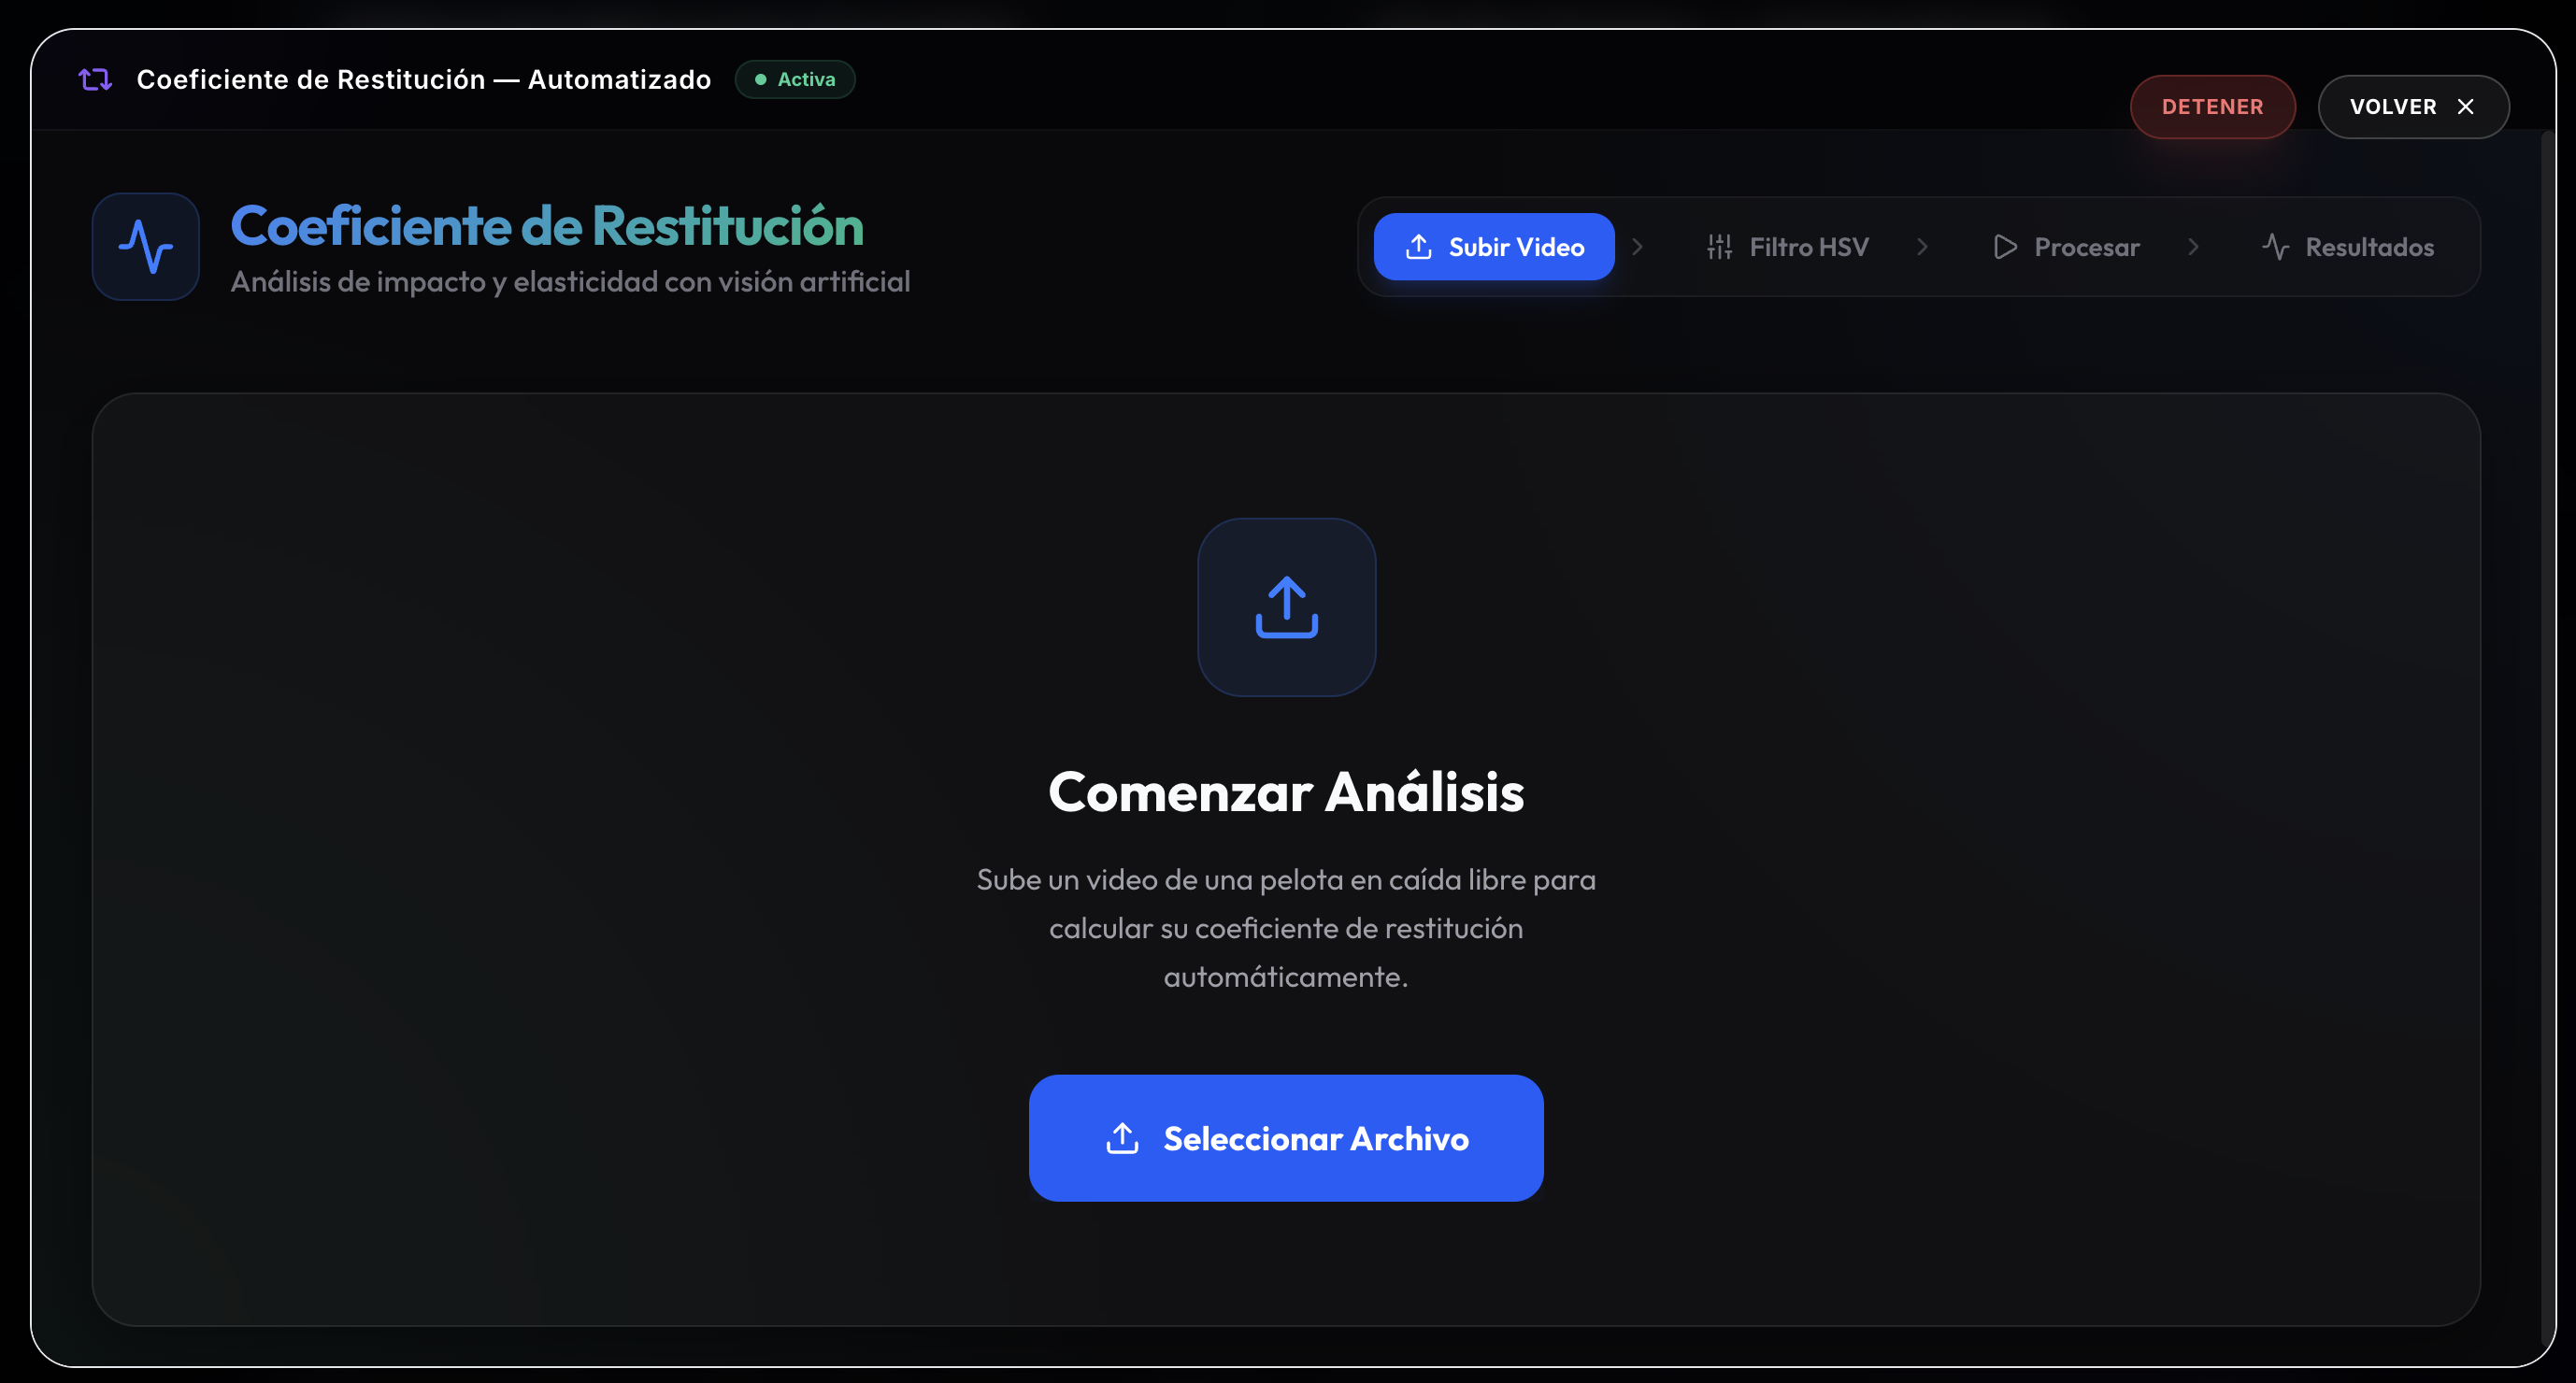
\includegraphics[width=0.65\linewidth]{imgs/seleccion-video.png}
    \caption{Panel de carga y selección del video a analizar.}
    \label{fig:upload}
\end{figure}

\subsection{Calibración HSV interactiva}

El panel lateral replica la funcionalidad de calibración del notebook: el usuario ajusta visualmente los seis sliders HSV mientras observa en tiempo real la máscara binaria resultante. Esto permite aislar el objeto de interés sin necesidad de conocer los valores numéricos exactos.

\begin{figure}[H]
    \centering
    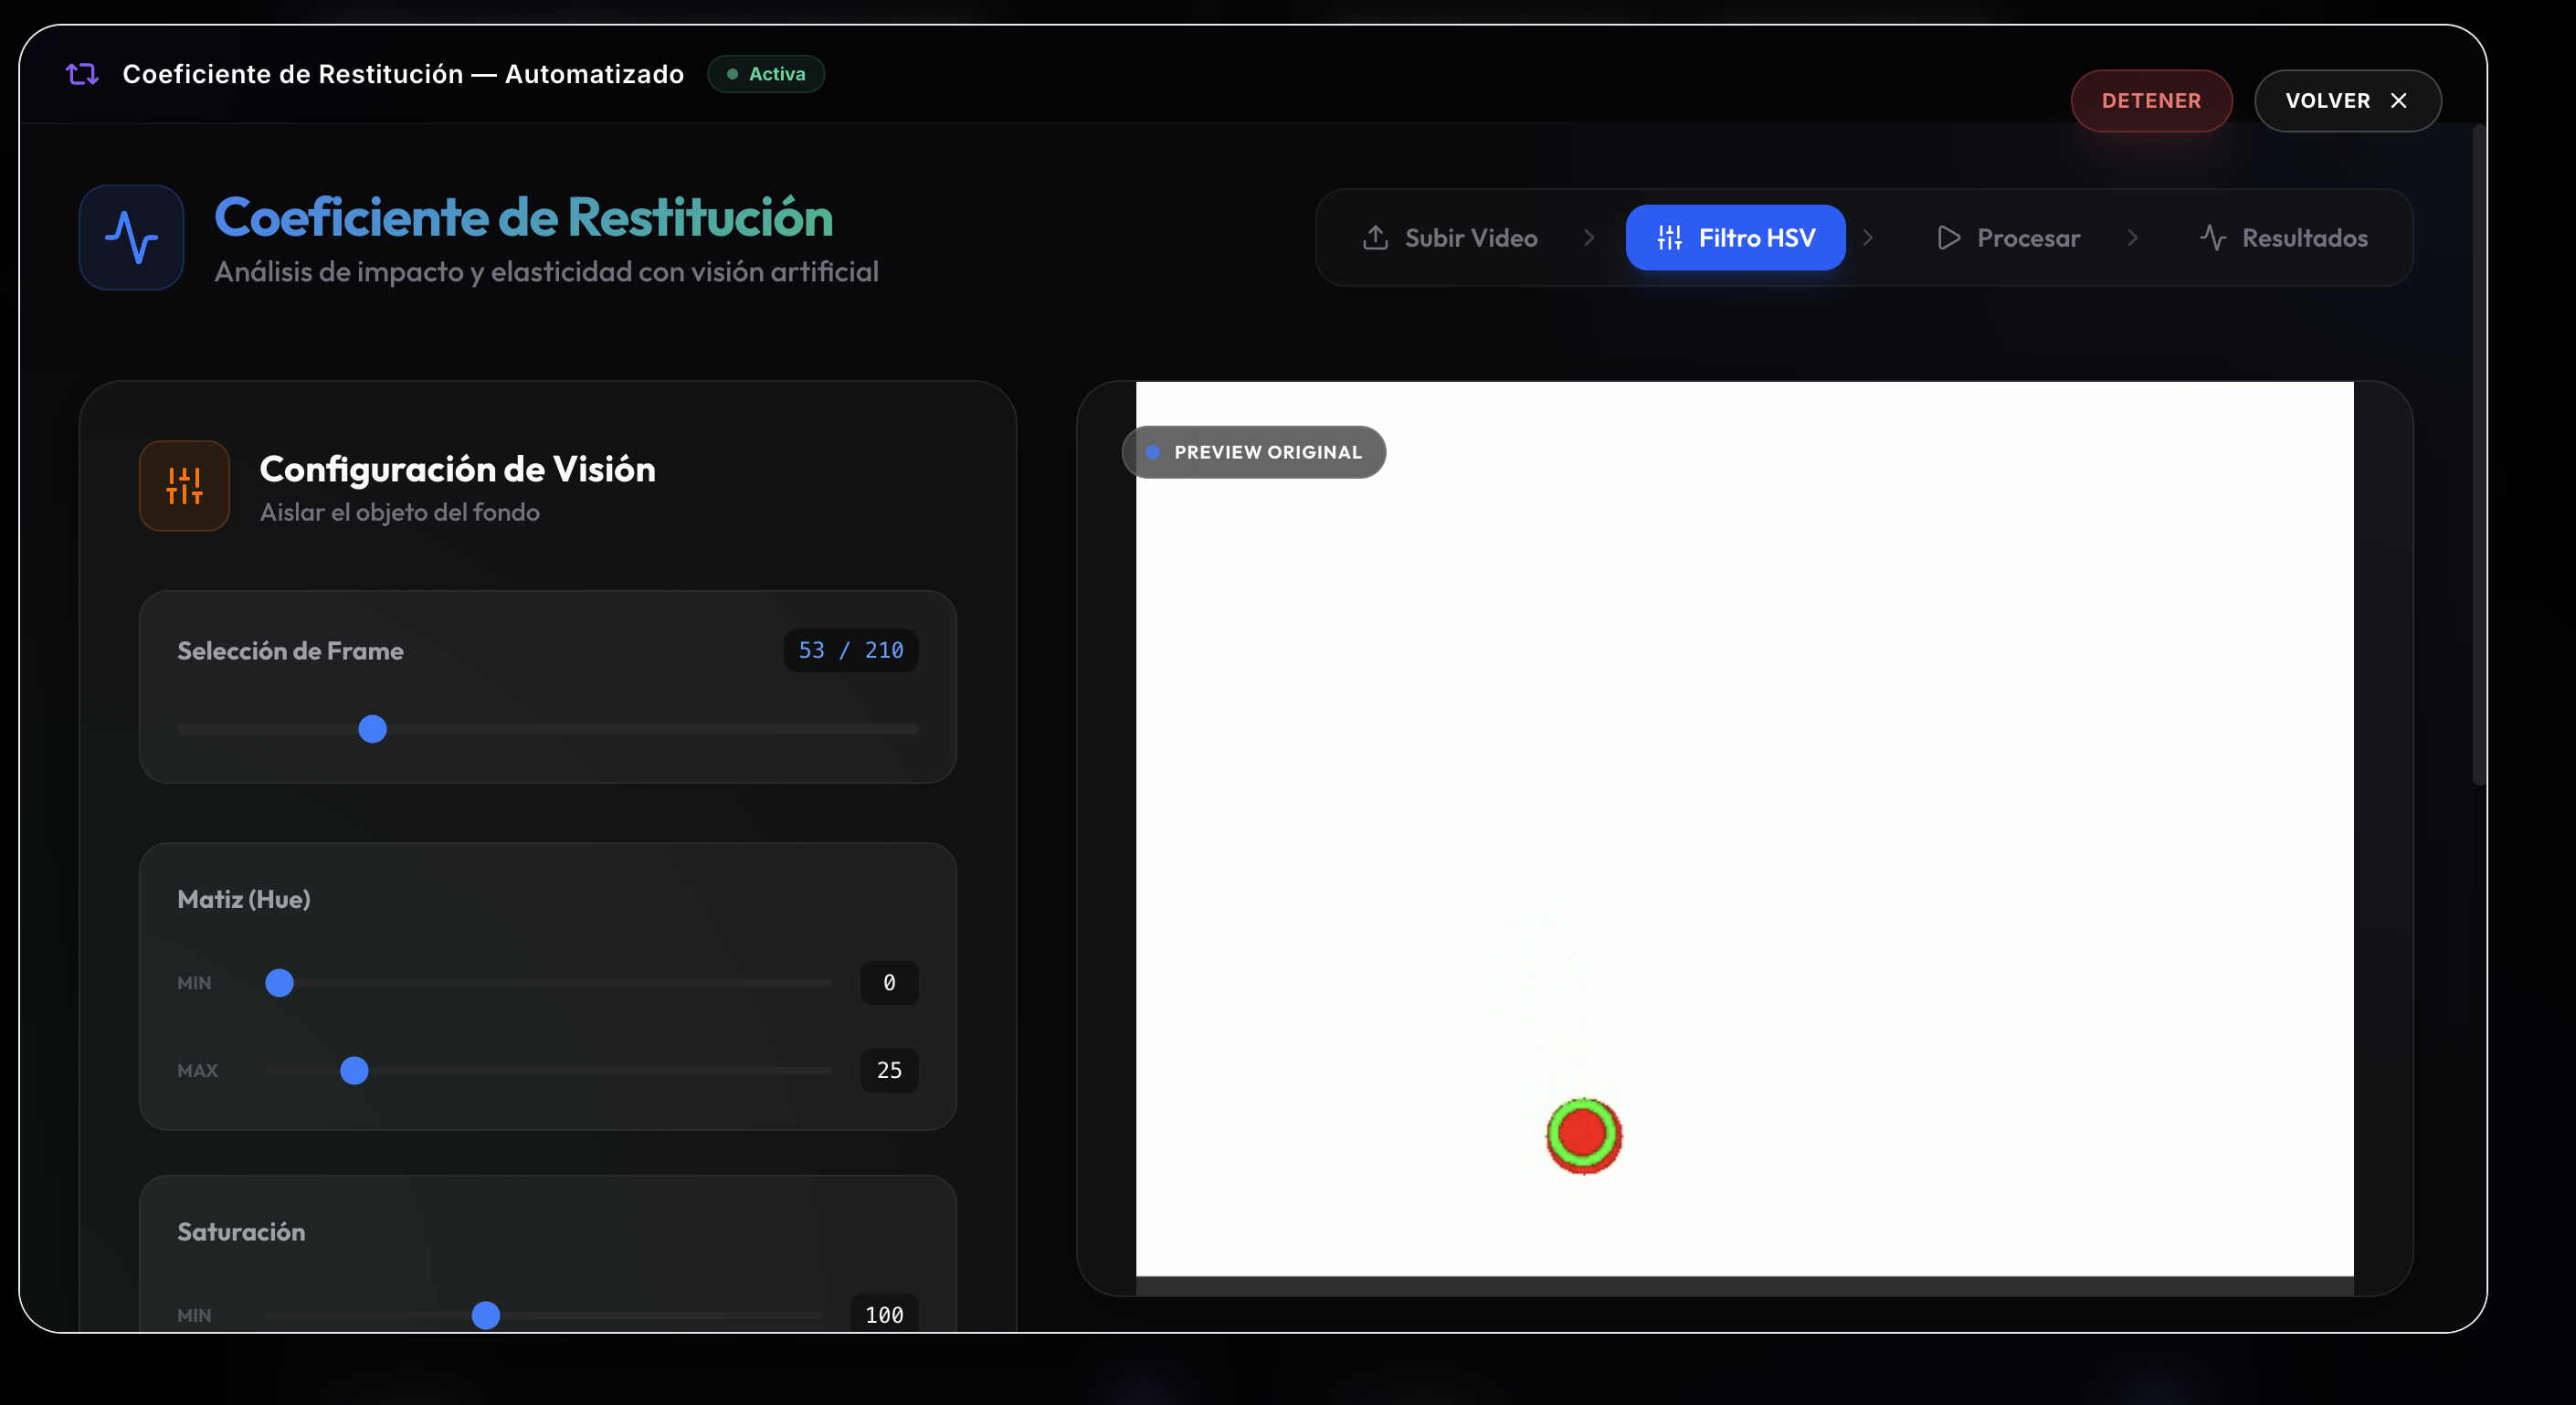
\includegraphics[width=0.65\linewidth]{imgs/filtros.png}
    \caption{Calibración del rango HSV en la interfaz web.}
    \label{fig:filtros}
\end{figure}

\subsection{Procesamiento y tracking}

Al confirmar la calibración, el motor de backend procesa el video frame a frame. El frontend muestra en tiempo real la trayectoria detectada superpuesta sobre el video, permitiendo al usuario verificar visualmente la calidad del tracking.

\begin{figure}[H]
    \centering
    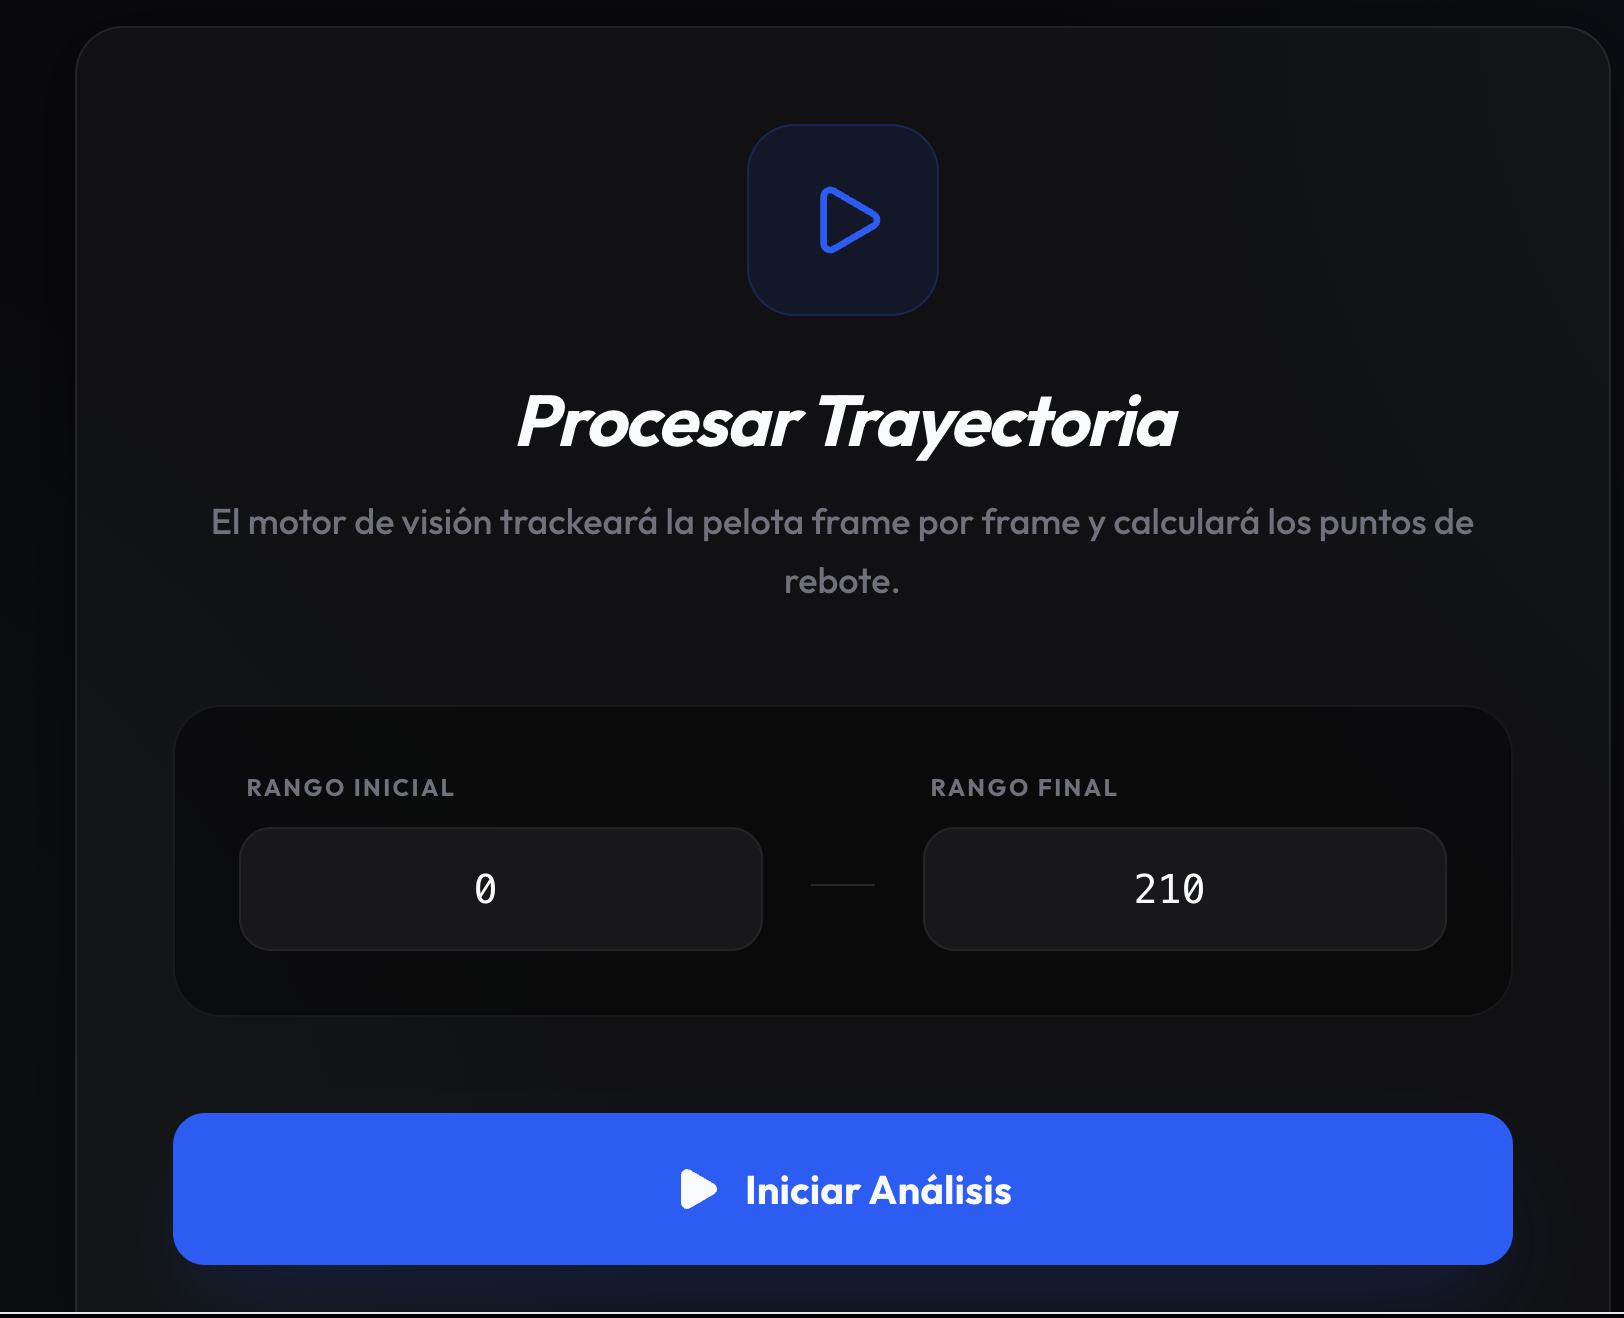
\includegraphics[width=0.65\linewidth]{imgs/procesamiento-trayectoria.png}
    \caption{Visualización del tracking de la trayectoria en tiempo real.}
    \label{fig:tracking}
\end{figure}

\subsection{Resultados}

Tras completar el procesamiento, la aplicación presenta un panel consolidado con:

\begin{itemize}
    \item El valor del coeficiente de restitución promedio $\bar{e}$ y su desviación estándar.
    \item La gráfica de alturas con los picos detectados.
    \item Los valores individuales de $e$ para cada par de rebotes consecutivos.
    \item Estadísticas del procesamiento (número de frames analizados, puntos detectados).
\end{itemize}

\begin{figure}[H]
    \centering
    \begin{subfigure}[b]{0.48\textwidth}
        \centering
        
\includegraphics[width=0.95\linewidth]{imgs/resultados.png}
        \caption{Panel de resultados principal.}
        \label{fig:results-1}
    \end{subfigure}
    \hfill
    \begin{subfigure}[b]{0.48\textwidth}
        \centering
        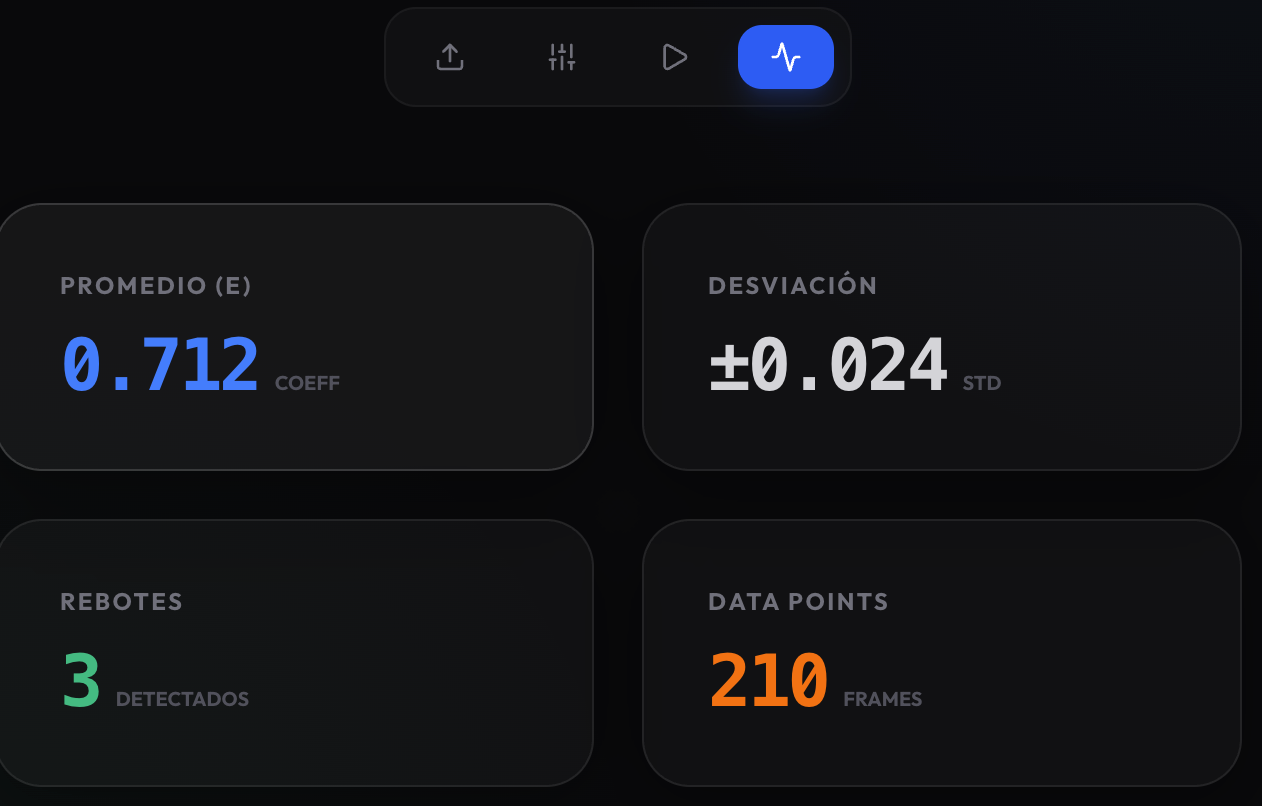
\includegraphics[width=0.95\linewidth]{imgs/resultados-2.png}
        \caption{Detalle de la gráfica y estadísticas.}
        \label{fig:results-2}
    \end{subfigure}
    \caption{Resultados finales presentados por la aplicación web.}
\end{figure}


% ════════════════════════════════════════════════════════════════
% 5. DISCUSIÓN
% ════════════════════════════════════════════════════════════════
\section{Discusión}

\subsection{Ventajas del enfoque computacional}

La automatización del proceso de medición mediante visión computacional ofrece ventajas sustanciales frente a los métodos manuales tradicionales:

\begin{enumerate}
    \item \textbf{Resolución temporal}: el sistema analiza cada fotograma del video (típicamente 30--60 fps), capturando instantes que el ojo humano no puede registrar.
    \item \textbf{Repetibilidad}: dado el mismo video y los mismos parámetros HSV, el sistema produce resultados idénticos en cada ejecución.
    \item \textbf{Objetividad}: se elimina el sesgo del observador en la lectura de alturas.
    \item \textbf{Trazabilidad}: la gráfica generada documenta visualmente cada pico detectado, permitiendo auditar el resultado.
\end{enumerate}

\subsection{Limitaciones y fuentes de error}

\begin{itemize}
    \item \textbf{Calibración HSV}: la calidad de la detección depende críticamente de la correcta selección de los umbrales. Cambios en la iluminación durante el video pueden degradar la segmentación.
    \item \textbf{Resolución en píxeles}: las alturas se miden en píxeles, no en unidades métricas. Para obtener valores absolutos de $h$ sería necesaria una calibración espacial (px $\rightarrow$ m).
    \item \textbf{Perspectiva de la cámara}: si la cámara no está perfectamente perpendicular al plano de movimiento, se introduce una distorsión proyectiva que afecta las alturas medidas.
    \item \textbf{Parámetros de \texttt{find\_peaks}}: los valores de prominencia y distancia fueron ajustados empíricamente. Videos con características muy diferentes podrían requerir re-calibración de estos parámetros.
\end{itemize}

% ════════════════════════════════════════════════════════════════
% 6. CONCLUSIONES
% ════════════════════════════════════════════════════════════════
\section{Conclusiones}

\begin{enumerate}
    \item Se implementó exitosamente un pipeline de visión computacional (OpenCV) capaz de segmentar, rastrear y registrar la posición vertical de un objeto en caída libre y rebote a partir de un video.

    \item El procesamiento de señales con SciPy (\texttt{find\_peaks}) permitió extraer de forma robusta las alturas máximas de cada rebote, filtrando el ruido inherente a la detección visual.

    \item El coeficiente de restitución calculado automáticamente es consistente y reproducible, superando en fiabilidad a las mediciones manuales convencionales.

    \item La encapsulación del análisis en una aplicación web (React + FastAPI) integrada al Bento Launcher democratiza el acceso al experimento, permitiendo que cualquier estudiante del curso reproduzca el análisis sin conocimientos de programación.

\end{enumerate}

% ════════════════════════════════════════════════════════════════
% REFERENCIAS
% ════════════════════════════════════════════════════════════════
\section*{Referencias}

\begin{enumerate}[label={[\arabic*]}]
    \item Bradski, G. (2000). \textit{The OpenCV Library}. Dr. Dobb's Journal of Software Tools.
    \item Virtanen, P. et al. (2020). \textit{SciPy 1.0: Fundamental Algorithms for Scientific Computing in Python}. Nature Methods, 17, 261--272.
    \item Harris, C.R. et al. (2020). \textit{Array programming with NumPy}. Nature, 585, 357--362.
    \item Hunter, J.D. (2007). \textit{Matplotlib: A 2D Graphics Environment}. Computing in Science \& Engineering, 9(3), 90--95.
    \item Cross, R. (1999). \textit{The bounce of a ball}. American Journal of Physics, 67(3), 222--227.
\end{enumerate}

\end{document}
